\documentclass[10pt,twoside]{article}
\usepackage[T1]{fontenc}
\usepackage{harvard}
\usepackage{url}
\usepackage{graphicx}
\graphicspath{ {../images/} }
\pagestyle{plain}

\def\all{all}
\ifx\files\all \typeout{Including all files.} \else %\typeout{Including only \files.} \includeonly{\files} \fi

% Keywords command
\providecommand{\keywords}[1]
{
  \small	
  \textbf{\textit{Keywords---}} #1
}

\title{Digital Sponsorship: Structured Literature Review}
\author{Pieter Joubert \\
	Vega School Bordeaux \\
	}

\date{\today}
% Hint: \title{what ever}, \author{who care} and \date{when ever} could stand 
% before or after the \begin{document} command 
% BUT the \maketitle command MUST come AFTER the \begin{document} command! 
\begin{document}

\maketitle
\keywords{Digital Sponsorship, Brand Leadership, Game Design, Game Development, Structured Literature Review.}

\section{Subject Area}
Brand Leadership and Management
\section{Introduction}

The field of digital sponsorship, specifically in the field of eSports, is one that requires further investigation, according to various authors \cite{huettermann2020esports}, \cite{Elasri-Ejjaberi2020}. Furthermore it is unclear to what extent game design and level design effect how gamers perceive brand placement in digital games \cite{hwang2017effects}.

This paper will thus explore the current state of the literature regarding Digital Sponsorship in eSports, and more specifically the link between Game and Level Design and Brand Placement in eSports.

The Research Question that this paper wishes to explore is: To what extent has the link between Game and Level Design and Brand Placement in eSports been explored in the literature?

\section{Literature}
The field of Digital Sponsorship is still nascent, but there is a growing body of literature exploring various aspects of Digital Sponsorship. Some authors are comparing Digital Sponsorship to traditional forms of Sports Sponsorship \cite{huettermann2020esports}, others are exploring the possibility of Brand Harm and Digital Sponsorship \cite{Freitas2019} and finally authors are generally commenting on the lack of detailed research within this field and performing their own exploratory literature reviews \cite{Elasri-Ejjaberi2020}.

To help underpin the study Aaker's Brand Identity model will be used to provide theoretical structure and classification to the literature reviewed and the summary of the literature that will be produced. \cite{aaker2012brand}

\section{Methodology and Data Analysis}

The research data, being academic literature can be classified as highly mediated, but unstructured, using the mixed methods framework of Plowright \cite{plowright2011using}. This classification naturally leads to performing a Structured Literature Review \cite{petticrew2008systematic}.

To ensure that the literature that is reviewed is structured into a logical format, Aaker's Brand Identity model will be used. The four brand identity perspectives (brand as a product, an organization, a person, and a symbol) will be used as the primary categories for classification \cite{aaker2012brand}. Each of these primary categories will then be sub-divided into the appropriate sub-category as shown below:

\begin{figure}[h]
\caption{Brand Identity Model Adapted from Aaker}
\centering
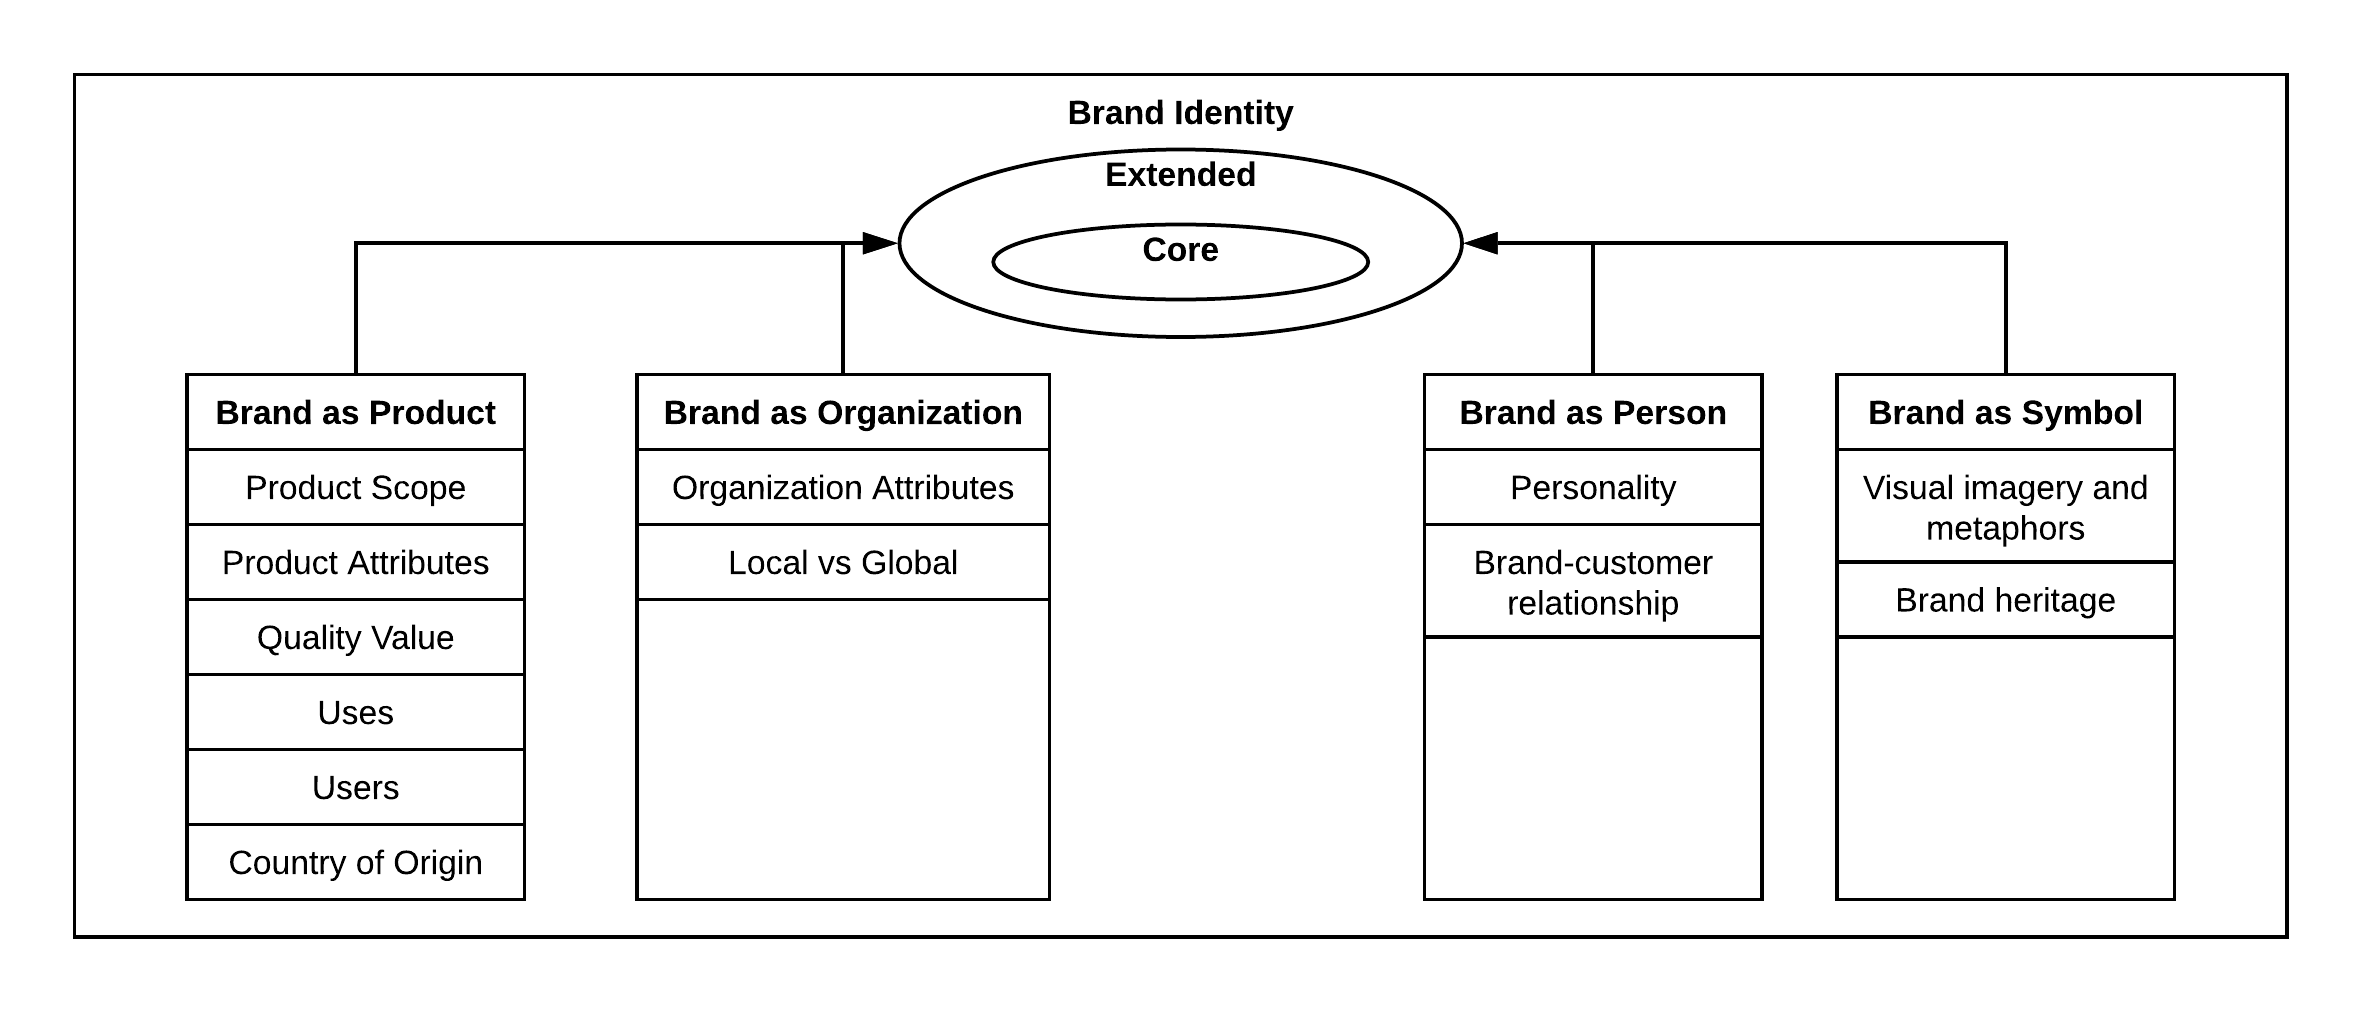
\includegraphics[width=1.2\textwidth]{BrandIdentityModel.png}
\end{figure}

This approach will link the sources reviewed to the theoretical framework of Aaker's Brand Identity model, and through doing so, identify any gaps in the literature.

\section{Ethical Clearance}
No participants of any kind will be included in the study so no ethical clearance will be required.

\section{Expected Findings and Results}
A clearer understanding of what research has been done in the field of Digital Sponsorship of eSports will be provided. This will hopefully also lead to the identification of any gaps within the literature, especially any concerning the link between Game and Level Design and Digital Sponsorship.

\section{Limitations of the Study}
The study will be time limited to explore the most recent literature in the field, and will be limited to eSports games only, to ensure that the study is focused.

\bibliographystyle{myharvard}
\bibliography{esports_slr, PHD_literature}

\end{document}
